\section{Multi-Layered Perceptrons} 

  We build upon what we already know: generalized linear models. In simple regression, we transform the inputs into the relevant features $\mathbf{x}_n \mapsto \boldsymbol{\phi} (\mathbf{x}_n) = \boldsymbol{\phi}_n$ and then, when we construct a generalized linear model, we assume that the conditional distribution $Y \mid X = x$ is in the canonical exponential family, with some natural parameter $\eta(x)$ and expected mean $\mu(x) = \mathbb{E}[Y \mid X = x]$. Then, to choose the link function $g$ that related $g(\mu(x)) = x^T \beta$, we can set it to be the canonical link $g$ that maps $\mu$ to $\eta$. That is, we have $g(\mu(x)) = x^T \beta = \eta (x)$ such that the natural parameter is linearly dependent on the input. The inverse $g^{-1}$ of the link function is called the \textbf{activation function}, which connects the expected mean to a linear function of $x$. 
  \begin{equation}
    h_\beta (x) = g^{-1} (x^T \beta) = \mu(x) = \mathbb{E}[Y \mid X = x]
  \end{equation}
  Now, note that for a classification problem, the decision boundary defined in the $\boldsymbol{\phi}$ feature space is linear, but it may not be linear in the input space $\mathcal{X}$. We would like to extend this model by making the basis functions $\boldsymbol{\phi}_n$ depend on the parameters $\mathbf{w}$ and then allow these parameters to be adjusted during training. 

  \begin{figure}[H]
    \centering
    \begin{subfigure}[t]{0.24\textwidth}
      \centering
      \includegraphics[width=\textwidth]{img/untrans_data.png}
      \caption{Data in space $\mathcal{X} = \mathbb{R}^2$.}
      \label{fig:raw_points}
    \end{subfigure}
    \hfill
    \begin{subfigure}[t]{0.24\textwidth}
      \centering
      \includegraphics[width=\textwidth]{img/trans_data.png}
      \caption{Transformed data $\phi(\mathbf{x}) = \|\mathbf{x}\|$.}
      \label{fig:transformed_points}
    \end{subfigure}
    \hfill
    \begin{subfigure}[t]{0.24\textwidth}
      \centering
      \includegraphics[width=\textwidth]{img/trans_fit.png}
      \caption{Logistic fit in transformed space.}
      \label{fig:transformed_trained}
    \end{subfigure}
    \hfill
    \begin{subfigure}[t]{0.24\textwidth}
      \centering
      \includegraphics[width=\textwidth]{img/untrans_fit.png}
      \caption{Logistic fit to data in input space.}
      \label{fig:raw_trained}
    \end{subfigure}
    \caption{Consider the set of points in $\mathbb{R}^2$ with the corresponding class. We transform the features to $\boldsymbol{\phi}(x_1, x_2) = x_1^2 + x_2^2$, which gives us a new space to work with. Fitting logistic regression onto this gives a linear decision boundary in the space $\boldsymbol{\phi}$, but the boundary is circular in $\mathcal{X} = \mathbb{R}^2$.}
    \label{fig:logistic_transformed}
  \end{figure}

\subsection{Feedforward Fully-Connected Networks}

  So how should we construct parametric nonlinear basis functions? One way is to have a similar architecture as GLMs by having a linear map followed by an activation function $f(x) = \sigma(w^T x + b)$. The simplest such function with the activation function as the step function 
  \begin{equation}
    f(z) = \begin{cases} 1 & \text{ if } z \geq 0 \\ 0 & \text{ if } z < 0 \end{cases}
  \end{equation}
  is the perceptron algorithm. It divides $\mathbb{R}^d$ using a hyperplane $\boldsymbol{\omega}^T \mathbf{x} + b = 0$ and linearly classifies all points on one side to value $1$ and the other side to value $0$. This is similar to a neuron, which takes in a value and outputs a ``signal" if the function evaluated gets past a threshold. However, for reasons regarding training these networks, we would like to use smooth activation functions for this, so we would use different activations. Hence we have a neuron. 

  \begin{definition}[Neuron]
    A \textbf{neuron} is a function of form 
    \begin{equation}
      y = \sigma(\mathbf{w}^T x  + b)
    \end{equation}
    where $\sigma: \mathbb{R} \rightarrow \mathbb{R}$ is any nonlinear function, called an \textbf{activation functions}. 
  \end{definition}
  
  Ultimately, a neural net is really just a generalized linear model with some trained feature extractors, which is why in practice, if researchers want to predict a smaller dataset, they take a pretrained model on a related larger dataset and simply tune the final layer, since the second last layer most likely encodes all the relevant features. This is called \textit{transfer learning}. But historically, it was called a \textit{multilayer perceptron} and the name stuck. 

  \begin{definition}[Feedforward, Fully-Connected Multilayer Perceptron]
    A $L$-layer \textbf{multilayer perceptron (MLP)} $f_\theta : \mathbb{R}^D \rightarrow \mathbb{R}^M$, with parameters $\theta$, is a function of form 
    \begin{equation}
      h_\theta (\mathbf{x}) \coloneqq \sigma^{[L]} \circ W^{[L]} \circ \sigma^{[L-1]} \circ W^{[L-1]} \circ \cdots \circ \sigma^{[1]} \circ W^{[1]} (\mathbf{x})
    \end{equation}
    where $\sigma^{[l]}: \mathbb{R}^{N^{[l]}} \rightarrow \mathbb{R}^{N^{[l]}}$ is an activation function and $W^{[l]}: \mathbb{R}^{N^{[l-1]}} \rightarrow \mathbb{R}^{N^{[l]}}$ is an affine map. We will use the following notation. 
    \begin{enumerate}
      \item The inputs will be labeled $\mathbf{x} = a^{[0]}$ which is in $\mathbb{R}^{N^{[0]}} = \mathbb{R}^D$. 
      
      \item We map $a^{[l]} \in \mathbb{R}^{N^{[l]}} \mapsto W^{[l+1]} a^{[l]} + b^{[l+1]}= z^{[l+1]} \in \mathbb{R}^{N^{[l+1]}}$, where $z$ denotes a vector after an affine transformation. 

      \item We map $z^{[l+1]} \in \mathbb{R}^{N^{[l+1]}} \mapsto \sigma(z^{[l+1]}) = a^{[l+1]} \in \mathbb{R}^{N^{[l+1]}}$, where $a$ denotes a vector after an activation function. 

      \item We keep doing this until we reach the second last layer with vector $a^{[L-1]}$. Note that in the last layer we do \textit{not} apply an activation function. 
    \end{enumerate}

    \begin{figure}[H]
      \centering 
      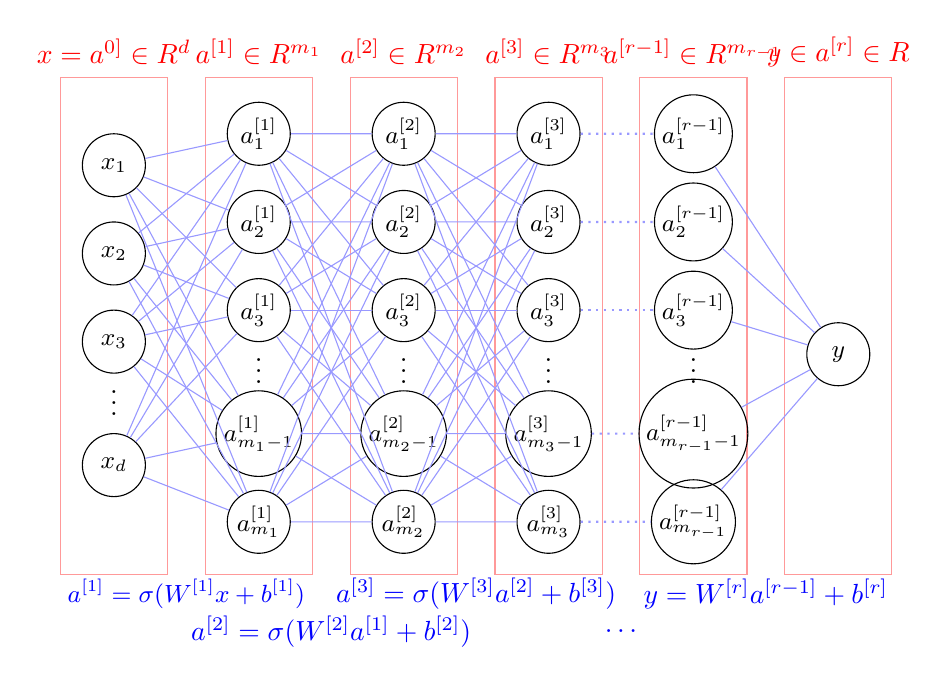
\begin{tikzpicture}[
        scale=0.8, 
        node distance=2cm,
        neuron/.style={circle, draw, minimum size=0.8cm, inner sep=1pt, font=\small},
        annotation/.style={text width=3cm},
        >=latex
      ]
        % Define some variables for consistent spacing
        \def\layersep{2.3}
        \def\neuronsep{1.4}
        \def\boxwidth{1.7}
        \def\boxheight{8}
        
        % Add dimension annotations above boxes in red
        \node[red] at (0, \boxheight/2 + 0.8) {$x = a^{0]} \in \mathbb{R}^d$};
        \node[red] at (\layersep, \boxheight/2 + 0.8) {$a^{[1]} \in \mathbb{R}^{m_1}$};
        \node[red] at (2*\layersep, \boxheight/2 + 0.8) {$a^{[2]} \in \mathbb{R}^{m_2}$};
        \node[red] at (3*\layersep, \boxheight/2 + 0.8) {$a^{[3]} \in \mathbb{R}^{m_3}$};
        \node[red] at (4*\layersep, \boxheight/2 + 0.8) {$a^{[r-1]} \in \mathbb{R}^{m_{r-1}}$};
        \node[red] at (5*\layersep, \boxheight/2 + 0.8) {$y \in a^{[r]} \in \mathbb{R}$};
        
        % Draw boxes
        \foreach \x in {0,1,2,3,4,5} {
            \draw[red!40] (\x*\layersep-\boxwidth/2, -\boxheight/2 + 0.5) rectangle (\x*\layersep+\boxwidth/2, \boxheight/2 + 0.4);
        }
        
        % Input layer (x) with adjusted vertical spacing
        \node[neuron] (x1) at (0, 3) {$x_1$};
        \node[neuron] (x2) at (0, {3-\neuronsep}) {$x_2$};
        \node[neuron] (x3) at (0, {3-2*\neuronsep}) {$x_3$};
        \node at (0, {3-2.6*\neuronsep}) {$\vdots$};
        \node[neuron] (xd) at (0, {3-3.4*\neuronsep}) {$x_d$};
        
        % Hidden layers with matching spacing pattern
        \foreach \l in {1,2,3} {
            \node[neuron] (a\l1) at (\l*\layersep, 3.5) {$a^{[\l]}_1$};
            \node[neuron] (a\l2) at (\l*\layersep, {3.5-\neuronsep}) {$a^{[\l]}_2$};
            \node[neuron] (a\l3) at (\l*\layersep, {3.5-2*\neuronsep}) {$a^{[\l]}_3$};
            \node at (\l*\layersep, {3.5-2.6*\neuronsep}) {$\vdots$};
            \node[neuron] (a\l m1) at (\l*\layersep, {3.5-3.4*\neuronsep}) {$a^{[\l]}_{m_{\l}-1}$};
            \node[neuron] (a\l m) at (\l*\layersep, {3.5-4.4*\neuronsep}) {$a^{[\l]}_{m_{\l}}$};
        }
        
        % Second-to-last layer (r-1)
        \node[neuron] (ar1) at (4*\layersep, 3.5) {$a^{[r-1]}_1$};
        \node[neuron] (ar2) at (4*\layersep, {3.5-\neuronsep}) {$a^{[r-1]}_2$};
        \node[neuron] (ar3) at (4*\layersep, {3.5-2*\neuronsep}) {$a^{[r-1]}_3$};
        \node at (4*\layersep, {3.5-2.6*\neuronsep}) {$\vdots$};
        \node[neuron] (arm1) at (4*\layersep, {3.5-3.4*\neuronsep}) {$a^{[r-1]}_{m_{r-1}-1}$};
        \node[neuron] (arm) at (4*\layersep, {3.5-4.4*\neuronsep}) {$a^{[r-1]}_{m_{r-1}}$};
        
        % Output layer
        \node[neuron] (y) at (5*\layersep, 0) {$y$};
        
        % Add σ annotations below connections
        \node[blue] at (0.5*\layersep, -3.8) {\small $a^{[1]} = \sigma(W^{[1]} x + b^{[1]})$};
        \node[blue] at (1.5*\layersep, -4.4) {$a^{[2]} = \sigma(W^{[2]} a^{[1]} + b^{[2]})$};
        \node[blue] at (2.5*\layersep, -3.8) {$a^{[3]} = \sigma(W^{[3]} a^{[2]} + b^{[3]})$};
        \node[blue] at (3.5*\layersep, -4.4) {$\ldots$};
        \node[blue] at (4.5*\layersep, -3.8) {$y = W^{[r]} a^{[r-1]} + b^{[r]}$};
        
        % Draw connections with thinner lines
        \begin{scope}[blue!40, thin]
            % From input to first hidden layer
            \foreach \i in {1,2,3,d} {
                \foreach \j in {1,2,3} {
                    \draw (x\i) -- (a1\j);
                }
                \draw (x\i) -- (a1m1);
                \draw (x\i) -- (a1m);
            }
            
            % Between visible hidden layers
            \foreach \l [remember=\l as \lastl (initially 1)] in {2,3} {
                \foreach \i in {1,2,3} {
                    \foreach \j in {1,2,3} {
                        \draw (a\lastl\i) -- (a\l\j);
                    }
                    \draw (a\lastl\i) -- (a\l m1);
                    \draw (a\lastl\i) -- (a\l m);
                }
                \draw (a\lastl m1) -- (a\l m);
                \draw (a\lastl m1) -- (a\l m1);
                \foreach \j in {1,2,3} {
                    \draw (a\lastl m1) -- (a\l\j);
                }
                \draw (a\lastl m) -- (a\l m);
                \draw (a\lastl m) -- (a\l m1);
                \foreach \j in {1,2,3} {
                    \draw (a\lastl m) -- (a\l\j);
                }
            }
            
            % Dotted connections between layer 3 and r-1
            \foreach \i/\j in {1/1,2/2,3/3} {
                \draw[dotted, thick] (a3\i) -- (ar\j);
            }
            \draw[dotted, thick] (a3m1) -- (arm1);
            \draw[dotted, thick] (a3m) -- (arm);
            
            % From second-to-last to output
            \foreach \i in {1,2,3} {
                \draw (ar\i) -- (y);
            }
            \draw (arm1) -- (y);
            \draw (arm) -- (y);
        \end{scope}
      \end{tikzpicture}
      \caption{If there does not exist any edge from a potential input $x$ to an output $y$, then this means that $x$ is not relevant in calculating $y$, i.e. the weight is $0$. However, we usually work with \textbf{fully-connected neural networks}, which means that every input is relevant to calculating every output, since we usually cannot make assumptions about which variables are relevant or not. }
      \label{fig:multilayer_neural_net}
    \end{figure}
  \end{definition}

  Note that each layer corresponds to how close a neuron is to the output. But really any neuron can be a function of any other neuron. For example, we can connect a neuron from layer $4$ back to a neuron of layer $1$. For now, we will consider networks that are restricted to a \textbf{feed-forward} architecture, in other words having no closed directed cycles. 

  \begin{code}[Parameters and Neural Nets in PyTorch] 
    At this point, you have learned the theory of MLPs. To actually implement them in PyTorch, look at this module \href{code/parameters.ipynb}{here}, which will tell you on how to construct linear maps and activations functions, and more importantly see how you can look at the weights, modify them, and see how they are initialized. You can then learn how to explore the weights and biases of a neural network. 
  \end{code}

\subsection{Forward and Back Propagation}

  Back in the supervised learning notes, we have gone through the derivation for linear, logistic, and softmax regression. It turns out that despite them having very different architectures, with a identity, sigmoid, and softmax activation function, our choice of loss to be the mean squared loss, the binary cross-entropy, and the cross-entropy loss, had given very cute formulas in computing the gradient of the loss. Unfortunately, the formulas do not get cute when we differentiate neural networks, but they do come in a very structured way. To gain intuition, I would recommend to go over the exercises at the end of the chapter labeled ECE 689 Fall 2021 Midterm. If you just use chain rule to do the calculations, you can see that they require us to compute all the intermediate $z^{(i)}$'s and the $a^{(i)}$'s, a process called \textit{forward propagation}, before we compute the gradients. 

  \begin{definition}[Forward Propagation]
    Given an MLP $f$ and an input $x$, the process of sequentially evaluating 
    \begin{equation}
      x = a^{[0]} \mapsto z^{[1]} \mapsto a^{[1]} \mapsto \ldots \mapsto z^{[L]} \mapsto a^{[L]} = f(x)
    \end{equation}
    is called \textbf{forward propagation}. 
  \end{definition} 

  When we want to compute the derivative of $f$. we can see that the intermediate partial derivatives in the chain rule are repeatedly used. That is, if we have layer $0 \leq l \leq L$, then to compute the derivative with respect to the $l$th layer we use the chain rule 
  \begin{equation}
    \frac{\partial f}{\partial z^{[l]}} = \frac{\partial f}{\partial z^{[l+1]}} \cdot \frac{z^{[l+1]}}{z^{[l]}}
  \end{equation}
  which requires us to know the derivative at the $(l+1)$th layer, along with the current values of $z^{[l]}, z^{[l+1]}$ to evaluate the derivatives at the current point. Therefore, we must complete forward propagation first and then compute \textit{backwards} from the result to the input to compute the gradients. 

  \begin{definition}[Backward Propagation]
    Given an MLP $f$ with input $x$ that has been forward propagated, the process of sequentially evaluating 
    \begin{equation}
      \frac{\partial f}{\partial a^{[L]}} \mapsto \frac{\partial f}{\partial z^{[L]}} \mapsto \ldots \mapsto \frac{\partial f}{\partial z^{[L]}}, 
    \end{equation}
    is called \textbf{backward propagation}, or \textbf{backprop}. 
  \end{definition}

  Backpropagation is not hard, but it is cumbersome notation-wise. What we really want to do is just compute a very long vector with all of its partials $\partial E / \partial \boldsymbol{\theta}$. 

  \begin{algo}[Backpropagation]
    To compute $\frac{\partial E_n}{\partial w_{ji}^{[l]}}$, it would be natural to split it up into a portion where $E_n$ is affected by the term before activation $\mathbf{z}^{[l]}$ and how that is affected by $w_{ji}^{[l]}$. The same goes for the bias terms. 
    \begin{equation}
      \frac{\partial E_n}{\partial w_{ji}^{[l]}} = \underbrace{\frac{\partial E_n}{\partial \mathbf{z}^{[l]}}}_{1 \times N^{[l]}} \cdot \underbrace{\frac{\partial \mathbf{z}^{[l]}}{\partial w_{ji}^{[l]}}}_{N^{[l]} \times 1} \text{ and } \frac{\partial E_n}{\partial b_{i}^{[l]}} = \underbrace{\frac{\partial E_n}{\partial \mathbf{z}^{[l]}}}_{1 \times N^{[l]}} \cdot \underbrace{\frac{\partial \mathbf{z}^{[l]}}{\partial b_{i}^{[l]}}}_{N^{[l]} \times 1}
    \end{equation}
    It helps to visualize that we are focusing on 
    \begin{equation}
      \mathbf{h}_{\boldsymbol{\theta}} (\mathbf{x}) = g\big( \ldots \sigma( \underbrace{\mathbf{W}^{[l]} \mathbf{a}^{[l-1]} + \mathbf{b}^{[l]}}_{\mathbf{z}^{[l]}} )  \ldots \big)
    \end{equation}
    We can expand $\mathbf{z}^{[l]}$ to get 
    \begin{equation}
      \mathbf{z}^{[l]} = \begin{pmatrix} w_{11}^{[l]} & \ldots & w_{1 N^{[l-1]}}^{[l]} \\ \vdots & \ddots & \vdots \\ w_{N^{[l]} 1}^{[l]} & \ldots & w_{N^{[l]} N^{[l-1]}}^{[l]} \end{pmatrix} 
      \begin{pmatrix} a^{[l-1]}_1 \\ \vdots \\ a^{[l-1]}_{N^{[l-1]}} \end{pmatrix} + \begin{pmatrix} b_1^{[l]} \\ \vdots \\ b_{N^{[l]}_{[l]}} \end{pmatrix}
    \end{equation}
    $w_{ji}^{[l]}$ will only show up in the $j$th term of $\mathbf{z}^{[l]}$, and so the rest of the terms in $\frac{\partial \mathbf{z}^{[l]}}{\partial w_{ji}^{[l]}}$ will vanish. The same logic applies to $\frac{\partial \mathbf{z}^{[l]}}{\partial b_{i}^{[l]}}$, and so we really just have to compute 
    \begin{equation}
      \frac{\partial E_n}{\partial w_{ji}^{[l]}} = \underbrace{\frac{\partial E_n}{\partial z^{[l]}_j}}_{1 \times 1} \cdot \underbrace{\frac{\partial z^{[l]}_j}{\partial w_{ji}^{[l]}}}_{1 \times 1} = \delta^{[l]}_j \cdot \frac{\partial z^{[l]}_j}{\partial w_{ji}^{[l]}} \text{ and } \frac{\partial E_n}{\partial b_{i}^{[l]}} = \underbrace{\frac{\partial E_n}{\partial z^{[l]}_j}}_{1 \times 1} \cdot \underbrace{\frac{\partial z^{[l]}_j}{\partial b_{i}^{[l]}}}_{1 \times 1} = \delta^{[l]}_j \cdot \frac{\partial z^{[l]}_j}{\partial b_{i}^{[l]}}
    \end{equation}
    where the $\delta_j^{[l]}$ is called the $j$th \textbf{error term} of layer $l$. If we look at the evaluated $j$th row, 
    \begin{equation}
      z_j^{[l]} = w_{j1}^{[l]} a_1^{[l-1]} + \ldots w_{j N^{[l-1]}} a^{[l-1]}_{N^{[l-1]}} + b_j^{[l]}
    \end{equation}
    We can clearly see that $\frac{\partial z^{[l]}_j}{\partial w_{ji}^{[l]}} = a_i^{[l-1]}$ and $\frac{\partial z^{[l]}_j}{\partial b_{i}^{[l]}} = 1$, which means that our derivatives are now reduced to 
    \begin{equation}
      \frac{\partial E_n}{\partial w_{ji}^{[l]}} = \delta_j^{[l]} a_i^{[l-1]}, \;\;\;\;\; \frac{\partial E_n}{\partial b_{i}^{[l]}} = \delta_j^{[l]}
    \end{equation}
    What this means is that we must know the intermediate values $\mathbf{a}^{[l-1]}$ beforehand, which is possible since we would compute them using forward propagation and store them in memory. Now note that the partial derivatives at this point have been calculated without any consideration of a particular error function or activation function. To calculate $\boldsymbol{\delta}^{[L]}$, we can simply use the chain rule to get 
    \begin{equation}
      \delta_j^{[L]} = \frac{\partial E_n}{\partial z_j^{[L]}} = \frac{\partial E_n}{\partial \mathbf{a}^{[L]}} \cdot \frac{\partial \mathbf{a}^{[L]}}{\partial z_j^{[L]}} = \sum_k \frac{\partial E_n}{\partial a_k^{[L]}} \cdot \frac{\partial a_k^{[L]}}{\partial z_j^{[L]}}
    \end{equation}
    which can be rewritten in the matrix notation
    \begin{equation}
      \boldsymbol{\delta}^{[L]} = \bigg( \frac{\partial \mathbf{g}}{\partial \mathbf{z}^{[L]}} \bigg)^T \bigg( \frac{\partial E_n}{\partial \mathbf{a}^{[L]}} \bigg) = \underbrace{\begin{bmatrix} \frac{\partial g_1}{\partial z_1^{[L]}} & \ldots & \frac{\partial g_{N^{[L]}}}{\partial z^{[L]}_1} \\ \vdots & \ddots & \vdots \\ \frac{\partial g_1}{\partial z^{[L]}_{N^{[L]}}} & \ldots & \frac{\partial g_{N^{[L]}}}{\partial z^{[L]}_{N^{[L]}}} \end{bmatrix}}_{N^{[L]} \times N^{[L]}} \begin{bmatrix} \frac{\partial E_n}{\partial a_1^{[L]}} \\ \vdots \\ \frac{\partial E_n}{\partial a_{N^{[L]}}^{[L]}} \end{bmatrix}
    \end{equation}
    Note that as soon as we make a model assumption on the form of the conditional distribution $Y \mid X = x$ (e.g. it is Gaussian), with it being in the exponential family, we immediately get two things: the loss function $E_n$ (e.g. sum of squares loss), and the canonical link function $\mathbf{g}$
    \begin{enumerate}
      \item If we assume that $Y \mid X = x$ is Gaussian in a regression (of scalar output) setting, then our canonical link would be $g(x) = x$, which gives the sum of squares loss function. Note that since the output is a real-valued scalar, $\mathbf{a}^{[L]}$ will be a scalar (i.e. the final layer is one node, $N^{[L]} = 1$). 
      \begin{equation}
        E_n = \frac{1}{2} (y^{(n)} - a^{[L]} )^2
      \end{equation}
      To calculate $\boldsymbol{\delta}^{[L]}$, we can simply use the chain rule to get 
      \begin{equation}
        \delta^{[L]} = \frac{\partial E_n}{\partial z^{[L]}} = \frac{\partial E_n}{\partial a^{[L]}} \cdot \frac{\partial a^{[L]}}{\partial z^{[L]}} = a^{[L]} - y^{(n)}
      \end{equation}

      \item For classification (of $M$ classes), we would use the softmax activation function (with its derivative next to it for convenience) 
      \begin{equation}
        \mathbf{g}(\mathbf{z}) = \mathbf{g} \bigg( \begin{bmatrix} z_1 \\ \vdots \\ z_M \end{bmatrix} \bigg) = \begin{bmatrix} e^{z_1} / \sum_k e^{z_k} \\ \vdots \\ e^{z_M} / \sum_k e^{z_k} \end{bmatrix}, \;\;\; \frac{\partial g_k}{\partial z_j} = \begin{cases} g_j (1 - g_j) & \text{ if } k = j \\ - g_j g_k & \text{ if } k \neq j \end{cases}
      \end{equation}
      which gives the cross entropy error 
      \begin{equation}
        E_n = - \mathbf{y}^{(n)} \cdot \ln \big( \mathbf{h}_{\boldsymbol{\theta}} (\mathbf{x}^{(n)}) \big) = -\sum_i y^{(n)}_i \, \ln(a_i^{[L]})
      \end{equation}
      where the $\mathbf{y}$ has been one-hot encoded into a standard unit vector in $\mathbb{R}^M$. To calculate $\boldsymbol{\delta}^{[L]}$, we can again use the chain rule again 
      \begin{align}
        \delta_j^{[L]} & = \sum_k \frac{\partial E_n}{\partial a_k^{[L]}} \cdot \frac{\partial a_k^{[L]}}{\partial z_j^{[L]}} \\
        & = - \sum_k \frac{y_k^{(n)}}{a_k^{{[L]}}} \cdot \frac{\partial a_k^{[L]}}{\partial z_j^{[L]}} \\
        & = \bigg( - \sum_{k \neq j} \frac{y_k^{(n)}}{a_k^{{[L]}}} \cdot \frac{\partial a_k^{[L]}}{\partial z_j^{[L]}} \bigg) - \frac{y_j^{(n)}}{a_j^{{[L]}}} \cdot \frac{a_j^{[L]}}{\partial z_j^{[L]}} \\ 
        & = \bigg( - \sum_{k \neq j} \frac{y_k^{(n)}}{a_k^{{[L]}}} \cdot - a_k^{[L]} a_j^{[L]} \bigg) - \frac{y_j^{(n)}}{a_j^{{[L]}}} \cdot a_j^{[L]} (1 - a_j^{[L]}) \\ 
        & = a_j^{[L]} \underbrace{\sum_{k} y_k^{(n)}}_{1} - y_j^{(n)} = a_j^{[L]} - y_j^{(n)}
      \end{align}
      giving us 
      \begin{equation}
        \boldsymbol{\delta}^{[L]} = \mathbf{a}_j^{[L]} - \mathbf{y}^{[L]}
      \end{equation}
    \end{enumerate}

    Now that we have found the error for the last layer, we can continue for the hidden layers. We can again expand by chain rule that 
    \begin{equation} 
      \delta_j^{[l]} = \frac{\partial E_n}{\partial z_j^{[l]}} = \frac{\partial E_n}{\partial \mathbf{z}^{[l+1]}} \cdot \frac{\partial \mathbf{z}^{[l+1]}}{\partial z_j^{[l]}} = \sum_{k=1}^{N^{[l+1]}} \frac{\partial E_n}{\partial z_k^{[l+1]}} \cdot \frac{\partial z_k^{[l+1]}}{\partial z_j^{[l]}} = \sum_{k=1}^{N^{[l+1]}} \delta_k^{[l+1]} \cdot \frac{\partial z_k^{[l+1]}}{\partial z_j^{[l]}}
    \end{equation} 
    By going backwards from the last layer, we should already have the values of $\delta_k^{[l+1]}$, and to compute the second partial, we recall the way $a$ was calculated 
    \begin{equation}
      z_k^{[l+1]} = b_k^{[l+1]} + \sum_{j=1}^{N^{[l]}} w_{kj}^{[l+1]} \sigma(z_j^{[l]}) \implies \frac{\partial z_k^{[l+1]}}{\partial z_j^{[l]}} = w_{kj}^{[l+1]} \cdot \sigma^\prime(z_j^{[l]})
    \end{equation}
    Now this is where the ``back" in backpropagation comes from. Plugging this into the equation yields a final equation for the error term in hidden layers, called the \textbf{backpropagation formula}: 
    \begin{equation}
      \delta_j^{[l]} = \sigma^\prime(z_j^{[l]}) \sum_{k=1}^{N^{[l+1]}} \delta_k^{[l+1]} \cdot w_{kj}^{[l+1]}
    \end{equation}
    which gives the matrix form 
    \begin{equation}
      \boldsymbol{\delta}^{[l]} = \boldsymbol{\sigma}^\prime (\mathbf{z}^{[l]}) \odot (\mathbf{W}^{[l+1]})^T \boldsymbol{\delta}^{[l+1]} = \begin{bmatrix} \sigma^\prime (z_1^{[l]}) \\ \vdots \\ \sigma^\prime (z_{N^{[L]}}^{[l]})\end{bmatrix} \odot \begin{bmatrix} w_{11}^{[l+1]} & \ldots & w^{[l+1]}_{N^{[l+1]} 1} \\ \vdots & \ddots & \vdots \\ w^{[l+1]}_{1 N^{[l]}} & \ldots & w^{[l+1]}_{N^{[l+1]} N^{[l]}} \end{bmatrix} \begin{bmatrix} \delta_1^{[l+1]} \\ \vdots \\ \delta_{N^{[l+1]}}^{[l+1]} \end{bmatrix} 
    \end{equation}
    and putting it all together, the partial derivative of the error function $E_n$ with respect to the weight in the hidden layers for $1 \leq l < L$ is 
    \begin{equation}
      \frac{\partial E_n}{\partial w_{ji}^{[l]}} = a_i^{[l-1]} \sigma^\prime(z_j^{[l]}) \sum_{k=1}^{N^{[l+1]}} \delta_k^{[l+1]} \cdot w_{kj}^{[l+1]} 
    \end{equation}
  \end{algo}

  A little fact is that the time complexity of both forward prop and back prop should be the same, so if you ever notice that the time to compute these two functions scales differently, you're probably making some repeated calculations somewhere. 

  \begin{algo}[Epoch of Training]
    Before training, we initialize all the parameters to be 
    \begin{equation}
      \boldsymbol{\theta} = (\mathbf{W}^{[1]}, \mathbf{b}^{[1]}, \mathbf{W}^{[2]}, \ldots, \mathbf{W}^{[L]}, \mathbf{b}^{[L]})
    \end{equation} 
    Then, we repeat the following for one epoch of training. 
    \begin{enumerate}
      \item \textit{Choose Batch}: We choose an arbitrary data point $(\mathbf{x}^{(n)}, \mathbf{y}^{(n)})$, an minibatch, or the entire batch to compute the gradients on. 
      
      \item \textit{Forward Propagation}: Apply input vector $\mathbf{x}^{(n)}$ and use forward propagation to compute the values of all the hidden and activation units 
      \begin{equation}
        \mathbf{a}^{[0]} = \mathbf{x}^{(n)}, \mathbf{z}^{[1]}, \mathbf{a}^{[1]}, \ldots, \mathbf{z}^{[L]}, \mathbf{a}^{[L]} = h_{\boldsymbol{\theta}} (\mathbf{x}^{(n)})
      \end{equation}
      
      \item \textit{Back Propagation}: 
      \begin{enumerate}
        \item Evaluate the $\boldsymbol{\delta}^{[l]}$'s starting from the back with the formula 
        \begin{align}
          \boldsymbol{\delta}^{[L]} & = \bigg( \frac{\partial \mathbf{g}}{\partial \mathbf{z}^{[L]}} \bigg)^T \bigg( \frac{\partial E_n}{\partial \mathbf{a}^{[L]}} \bigg) \\
          \boldsymbol{\delta}^{[l]} & = \boldsymbol{\sigma}^\prime (\mathbf{z}^{[l]}) \odot (\mathbf{W}^{[l+1]})^T \boldsymbol{\delta}^{[l+1]} \;\;\;\;\; l = 1, \ldots, L-1
        \end{align}
        where $\frac{\partial \mathbf{g}}{\partial \mathbf{z}^{[L]}}$ can be found by taking the derivative of the known link function, and the rest of the terms are found by forward propagation (these are all functions which have been fixed in value by inputting $\mathbf{x}^{(n)}$).  

        \item Calculate the derivatives of the error as 
        \begin{equation}
          \frac{\partial E_n}{\partial \mathbf{W}^{[l]}} = \boldsymbol{\delta}^{[l]} (\mathbf{a}^{[l-1]})^T, \;\;\;\;\; \frac{\partial E_n}{\partial \mathbf{b}^{[l]}} = \boldsymbol{\delta}^{[l]}
        \end{equation}
      \end{enumerate}
      
      \item \textit{Gradient Descent}: Subtract the derivatives with step size $\alpha$. That is, for $l = 1, \ldots, L$, 
      \begin{equation}
        \mathbf{W}^{[l]} = \mathbf{W}^{[l]} - \alpha \frac{\partial E_n}{\partial \mathbf{W}^{[l]}} , \;\;\;\;\; \mathbf{b}^{[l]} = \mathbf{b}^{[l]} - \alpha \frac{\partial E_n}{\partial \mathbf{b}^{[l]}}
      \end{equation}
      The specific optimizer can differ, e.g. Adam, SGD, BFGS, etc., but the specific algorithm won't be covered here. It is common to use Adam, since it usually works better. If we can afford to iterate over the entire batch, L-BFGS may also be useful. 
    \end{enumerate}
  \end{algo}

  \begin{code}[Neural Net from Scratch]
    Now it's time to implement what most newcomers fear most: a neural net from scratch using only numpy. Doing this will get you to understand the inner workings of a neural net, and you can find the relevant code \href{code/mlp_from_scratch.ipynb}{here}.  
  \end{code} 

  \begin{code}[Pytorch Implementation of Forward and Backward Propagation]
    Once you have finished implementing from scratch, you can now use the PyTorch API to access the same model weights. The code \href{code/forward_backward.ipynb}{here} shows how to look at the forward propagation and backpropagation steps in PyTorch in intermediate layers and shows the backend behind storing gradients. 
  \end{code}

